\section{Experimental Results}

\subsection{Generate Merkle tree}
\begin{frame}{Experimental Results}
	\begin{table}[]
		\scriptsize
		\centering
		\begin{tabular}{crcc}
			  & Size    & File  & Directory \\
			  &			&		&		    \\
			A & 777 MB  & 48    & 6         \\
			B & 145 MB  & 54198 & 188       \\
			C & 5.95 GB & 45089 & 1459      \\
		\end{tabular}
        
		\caption{GENERATE MERKLE TREE'S TIME (IN SEC.)}
		\begin{tabular}{|c|c|c|r|}
			\hline
              & Non Hashed & Pre Hashed & Merkle tree Size \\ \hline
            A & 9.40653    & 0.00132    & 5.4 KB           \\ \hline
            B & 55.14738   & 4.2467     & 5.08 MB          \\ \hline
            C & 339.18192  & 0.3342     & 4.37 MB          \\ \hline
		\end{tabular}
        
        \caption{SERIALIZE \& DESERIALIZE MERKLE TREE OBJECT'S TIME (IN SEC.)}
		\begin{tabular}{|c|c|c|}
            \hline
              & Serialize & Deserialize \\ \hline
            A & 0.04      & 0.009       \\ \hline
            B & 0.756     & 0.299       \\ \hline
            C & 0.67      & 0.295       \\ \hline
		\end{tabular}
	\end{table}
\end{frame}

\subsection{Non POV}
\begin{frame}{Experimental Results}{Non POV}
	\tiny
    \begin{table}[]
        \centering
        \begin{minipage}[c]{0.5\textwidth}
            \caption{The client device and SP are \newline in the same network segment}
            \begin{tabular}{lcc}
                                 & Upload (sec.) & Download (sec.) \\ \hline
                \textless 10 KB  & 0.010608      & 0.007845        \\ \hline
                \textless 100 KB & 0.014393      & 0.013691        \\ \hline
                \textless 1 MB   & 0.090440      & 0.088570        \\ \hline
                \textless 10 MB  & 0.367989      & 0.354916        \\ \hline
            \end{tabular}
            \begin{center}
                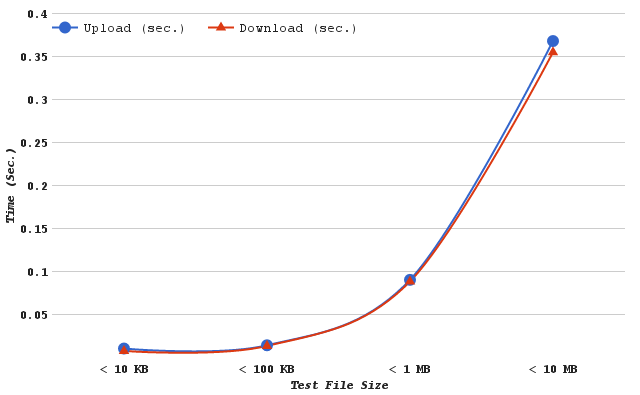
\includegraphics[width=\textwidth]{non_pov_same}
            \end{center}
        \end{minipage}%
        \begin{minipage}[c]{0.5\textwidth}
            \caption{The client device and SP are \newline \alert{not} in the same network segment}
            \begin{tabular}{lcc}
                                 & Upload (sec.) & Download (sec.) \\ \hline
                \textless 10 KB  & 0.069273      & 0.056629        \\ \hline
                \textless 100 KB & 0.121093      & 0.087351        \\ \hline
                \textless 1 MB   & 0.343584      & 0.225566        \\ \hline
                \textless 10 MB  & 1.675616      & 0.699524        \\ \hline
            \end{tabular}
            \begin{center}
                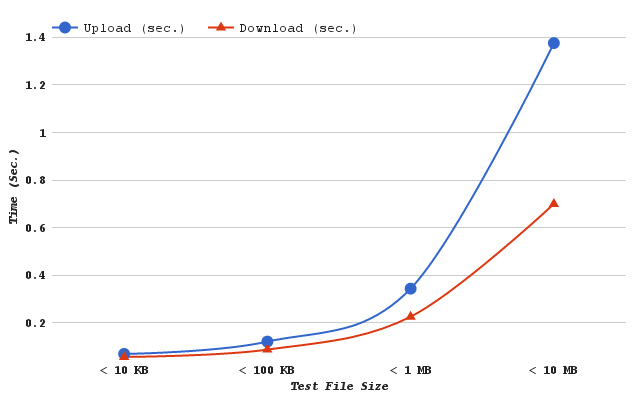
\includegraphics[width=\textwidth]{non_pov_not_same}
            \end{center}
        \end{minipage}
    \end{table}
\end{frame}

\subsection{Same Network Segment}
\begin{frame}{Experimental Results}
{The client device and SP are in the same network segment - My Method}
	\scriptsize
    \begin{table}[]
    \centering
    \caption{THE EXECUTION TIME OF \alert{UPLOAD} OPERATIONS (IN SEC.) (Account C)}
    \begin{tabular}{lcccc}
                         & 3 Server & 5 Server & 7 Server & 9 Server \\ \hline
        \textless 10 KB  & 0.046139 & 0.067923 & 0.101676 & 0.108696 \\ \hline
        \textless 100 KB & 0.070739 & 0.083563 & 0.112895 & 0.145049 \\ \hline
        \textless 1 MB   & 0.153822 & 0.166289 & 0.200053 & 0.203870 \\ \hline
        \textless 10 MB  & 0.430937 & 0.513879 & 0.684666 & 0.694259 \\ \hline
    \end{tabular}
    \end{table}
    \begin{center}
		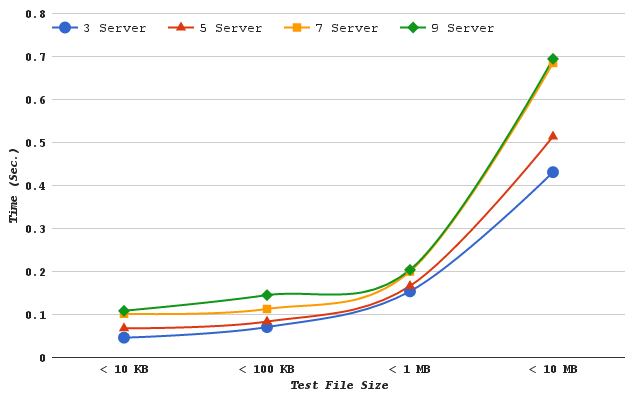
\includegraphics[width=.6\textwidth]{my_upload_same}
    \end{center}
\end{frame}

\begin{frame}{Experimental Results}
{The client device and SP are in the same network segment - My Method}
	\scriptsize
    \begin{table}[]
    \centering
    \caption{THE EXECUTION TIME OF \alert{DOWNLOAD} OPERATIONS (IN SEC.) (Account C)}
    \begin{tabular}{lcccc}
                         & 3 Server & 5 Server & 7 Server & 9 Server \\ \hline
        \textless 10 KB  & 0.042295 & 0.054263 & 0.064370 & 0.078872 \\ \hline
        \textless 100 KB & 0.053583 & 0.055442 & 0.083961 & 0.097507 \\ \hline
        \textless 1 MB   & 0.146021 & 0.159869 & 0.195817 & 0.202213 \\ \hline
        \textless 10 MB  & 0.392072 & 0.476251 & 0.622665 & 0.625499 \\ \hline
    \end{tabular}
    \end{table}
    \begin{center}
		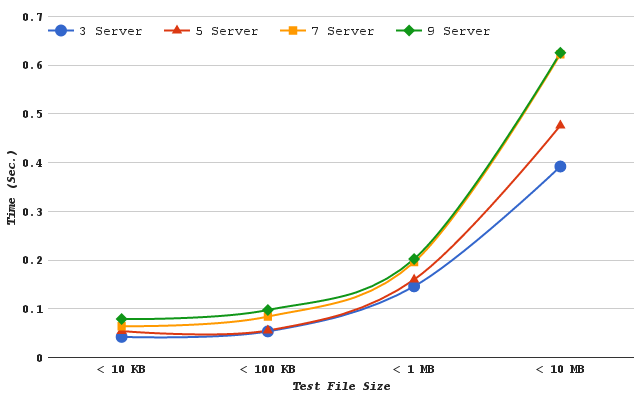
\includegraphics[width=.6\textwidth]{my_download_same}
    \end{center}
\end{frame}

\begin{frame}{Experimental Results}
{The client device and SP are in the same network segment - 2014 Cloud Com}
	\scriptsize
    \begin{table}[]
    \centering
    \caption{THE EXECUTION TIME OF \alert{UPLOAD} OPERATIONS (IN SEC.) (Account C)}
    \begin{tabular}{lccccl}
                         & sync 2   & sync 10  & sync 50  & sync 250 & sync 1250 \\ \hline
        \textless 10 KB  & 0.146783 & 0.184138 & 0.332988 & 0.486858 & 2.139086  \\ \hline
        \textless 100 KB & 0.194642 & 0.209044 & 0.341408 & 0.562457 & 2.147664  \\ \hline
        \textless 1 MB   & 0.331595 & 0.385494 & 0.403481 & 0.580193 & 2.251284  \\ \hline
        \textless 10 MB  & 0.501692 & 0.518835 & 0.576403 & 0.819175 & 2.409135  \\ \hline
    \end{tabular}
    \end{table}
    \begin{center}
		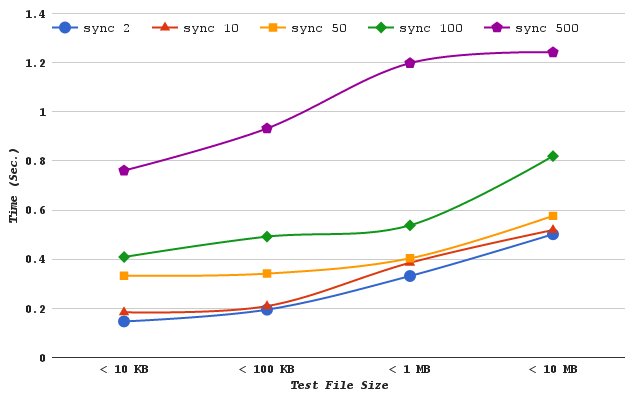
\includegraphics[width=.6\textwidth]{2014_upload_same}
    \end{center}
\end{frame}

\begin{frame}{Experimental Results}
{The client device and SP are in the same network segment - 2014 Cloud Com}
	\scriptsize
    \begin{table}[]
    \centering
    \caption{THE EXECUTION TIME OF \alert{DOWNLOAD} OPERATIONS (IN SEC.) (Account C)}
    \begin{tabular}{lccccl}
                         & sync 2   & sync 10  & sync 50  & sync 250 & sync 1250 \\ \hline
        \textless 10 KB  & 0.121268 & 0.249803 & 0.331339 & 0.937337 & 4.175263  \\ \hline
        \textless 100 KB & 0.134563 & 0.258717 & 0.338794 & 0.963107 & 4.211038  \\ \hline
        \textless 1 MB   & 0.279563 & 0.302230 & 0.440841 & 1.174882 & 4.294038  \\ \hline
        \textless 10 MB  & 0.462677 & 0.539638 & 0.595140 & 1.247275 & 4.360539  \\ \hline
    \end{tabular}
    \end{table}
    \begin{center}
		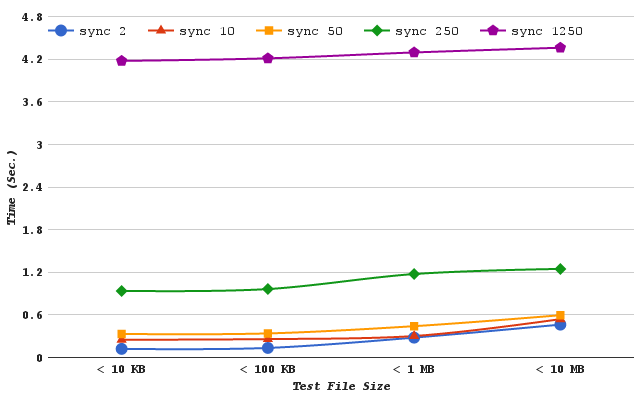
\includegraphics[width=.6\textwidth]{2014_download_same}
    \end{center}
\end{frame}

\begin{frame}{Experimental Results}
{The client device and SP are in the same network segment - UPLOAD operation}
	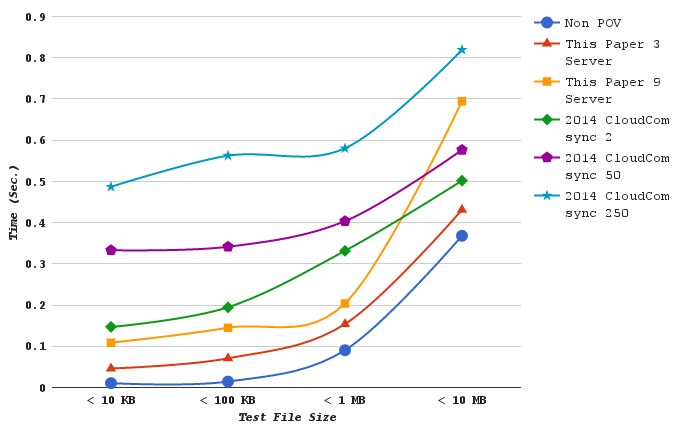
\includegraphics[width=\textwidth]{all_upload_same}
\end{frame}

\begin{frame}{Experimental Results}
{The client device and SP are in the same network segment - DOWNLOAD operation}
	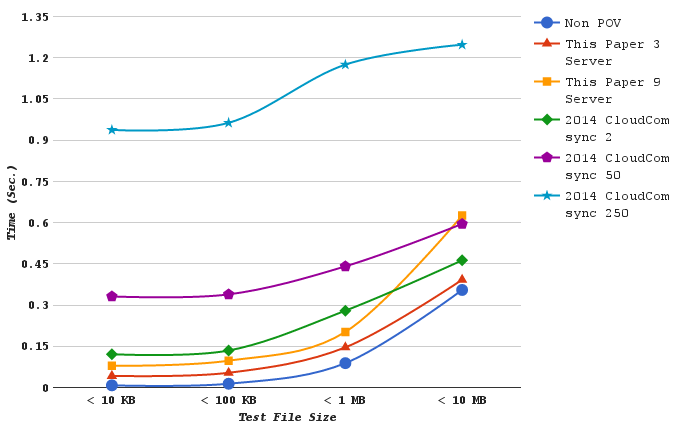
\includegraphics[width=\textwidth]{all_download_same}
\end{frame}

%OVERHEAD
\begin{frame}{Experimental Results}
{The client device and SP are in the same network segment - UPLOAD Overhead}
	\scriptsize
    \begin{table}[]
    \centering
    \caption{My Method - Non POV (IN SEC.) (Account C)}
    \begin{tabular}{lcccc}
     					 & 3 Server & 5 Server & 7 Server & 9 Server \\ \hline
        \textless 10 KB  & 0.035532 & 0.057315 & 0.091068 & 0.098088 \\ \hline
        \textless 100 KB & 0.056346 & 0.069170 & 0.098502 & 0.130656 \\ \hline
        \textless 1 MB   & 0.063382 & 0.075848 & 0.109612 & 0.113430 \\ \hline
        \textless 10 MB  & 0.062948 & 0.145890 & 0.316677 & 0.326270 \\ \hline
    \end{tabular}
    \caption{2014 Cloud Com - Non POV (IN SEC.) (Account C)}
    \begin{tabular}{lccccl}
       					 & sync 2   & sync 10  & sync 50  & sync 250 & sync 1250 \\ \hline
        \textless 10 KB  & 0.136175 & 0.173530 & 0.322380 & 0.476250 & 2.128478  \\ \hline
        \textless 100 KB & 0.180249 & 0.194651 & 0.327016 & 0.548064 & 2.133271  \\ \hline
        \textless 1 MB   & 0.241154 & 0.295053 & 0.313041 & 0.489752 & 2.160844  \\ \hline
        \textless 10 MB  & 0.133703 & 0.150846 & 0.208414 & 0.451186 & 2.041146  \\ \hline
    \end{tabular}
    \end{table}
\end{frame}

\begin{frame}{Experimental Results}
{The client device and SP are in the same network segment - DOWNLOAD Overhead}
	\scriptsize
    \begin{table}[]
    \centering
    \caption{My Method - Non POV (IN SEC.) (Account C)}
    \begin{tabular}{lcccc}
       					 & 3 Server & 5 Server & 7 Server & 9 Server \\ \hline
        \textless 10 KB  & 0.034450 & 0.046418 & 0.056526 & 0.071027 \\ \hline
        \textless 100 KB & 0.039892 & 0.041751 & 0.070270 & 0.083816 \\ \hline
        \textless 1 MB   & 0.057451 & 0.071299 & 0.107247 & 0.113643 \\ \hline
        \textless 10 MB  & 0.037156 & 0.121335 & 0.267749 & 0.270583 \\ \hline
    \end{tabular}
    \caption{2014 Cloud Com - Non POV (IN SEC.) (Account C)}
    \begin{tabular}{lccccl}
       					 & sync 2   & sync 10  & sync 50  & sync 250 & sync 1250 \\ \hline
        \textless 10 KB  & 0.113424 & 0.241959 & 0.323494 & 0.929492 & 4.167419  \\ \hline
        \textless 100 KB & 0.120872 & 0.245026 & 0.325103 & 0.949416 & 4.197347  \\ \hline
        \textless 1 MB   & 0.190993 & 0.213660 & 0.352271 & 1.086312 & 4.205468  \\ \hline
        \textless 10 MB  & 0.107761 & 0.184722 & 0.240224 & 0.892359 & 4.005623  \\ \hline
    \end{tabular}
    \end{table}
\end{frame}

%TIMES
\begin{frame}{Experimental Results}
{The client device and SP are in the same network segment - UPLOAD Overhead}
	\scriptsize
    \begin{table}[]
    \centering
    \caption{My Method / Non POV (IN SEC.) (Account C)}
    \begin{tabular}{lcccc}
                         & 3 Server & 5 Server & 7 Server & 9 Server  \\ \hline
        \textless 10 KB  & 4.349552 & 6.403042 & 9.584967 & 10.246768 \\ \hline
        \textless 100 KB & 4.914887 & 5.805870 & 7.843824 & 10.077857 \\ \hline
        \textless 1 MB   & 1.700816 & 1.838656 & 2.211983 & 2.254196  \\ \hline
        \textless 10 MB  & 1.171060 & 1.396453 & 1.860562 & 1.886630  \\ \hline
    \end{tabular}
    \caption{2014 Cloud Com / Non POV (IN SEC.) (Account C)}
    \begin{tabular}{lccccl}
                         & sync 2    & sync 10   & sync 50   & sync 250  & sync 1250  \\ \hline
        \textless 10 KB  & 13.837201 & 17.358624 & 31.390677 & 45.895962 & 201.651193 \\ \hline
        \textless 100 KB & 13.523544 & 14.524231 & 23.720780 & 39.079062 & 149.217959 \\ \hline
        \textless 1 MB   & 3.666447  & 4.262410  & 4.461293  & 6.415199  & 24.892477  \\ \hline
        \textless 10 MB  & 1.363336  & 1.409920  & 1.566359  & 2.226087  & 6.546762   \\ \hline
    \end{tabular}
    ~\\
    ~\\
    ~\\
    \alert{Avg: 6.61 times, Max: 19.67 times}
    \end{table}
\end{frame}

\begin{frame}{Experimental Results}
{The client device and SP are in the same network segment - DOWNLOAD Overhead}
	\scriptsize
    \begin{table}[]
    \centering
    \caption{My Method / Non POV (IN SEC.) (Account C)}
    \begin{tabular}{lcccc}
                         & 3 Server & 5 Server & 7 Server & 9 Server  \\ \hline
        \textless 10 KB  & 5.391663 & 6.917309 & 8.205786 & 10.054378 \\ \hline
        \textless 100 KB & 3.913722 & 4.049482 & 6.132484 & 7.121880  \\ \hline
        \textless 1 MB   & 1.648657 & 1.805003 & 2.210875 & 2.283095  \\ \hline
        \textless 10 MB  & 1.104689 & 1.341869 & 1.754401 & 1.762387  \\ \hline
    \end{tabular}
    \caption{2014 Cloud Com / Non POV (IN SEC.) (Account C)}
    \begin{tabular}{lccccl}
                         & sync 2    & sync 10   & sync 50   & sync 250   & sync 1250  \\ \hline
        \textless 10 KB  & 15.459033 & 31.844389 & 42.238325 & 119.489570 & 532.253193 \\ \hline
        \textless 100 KB & 9.828453  & 18.896670 & 24.745459 & 70.345135  & 307.573438 \\ \hline
        \textless 1 MB   & 3.156419  & 3.412343  & 4.977329  & 13.265056  & 48.482022  \\ \hline
        \textless 10 MB  & 1.303623  & 1.520467  & 1.676847  & 3.514280   & 12.286111  \\ \hline
    \end{tabular}
    ~\\
    ~\\
    ~\\
    \alert{Avg: 15.41 times, Max: 52.93 times}
    \end{table}
\end{frame}

\subsection{Not Same Network Segment}
\begin{frame}{Experimental Results}
{The client device and SP are \alert{not} in the same network segment - My Method}
	\scriptsize
    \begin{table}[]
    \centering
    \caption{THE EXECUTION TIME OF \alert{UPLOAD} OPERATIONS (IN SEC.) (Account C)}
    \begin{tabular}{lcccc}
                         & 3 Server & 5 Server & 7 Server & 9 Server \\ \hline
        \textless 10 KB  & 0.217563 & 0.331341 & 0.466655 & 0.570460 \\ \hline
        \textless 100 KB & 0.245769 & 0.410174 & 0.479227 & 0.660178 \\ \hline
        \textless 1 MB   & 0.433338 & 0.594532 & 0.640597 & 0.786688 \\ \hline
        \textless 10 MB  & 1.636473 & 1.972134 & 2.011500 & 2.163858 \\ \hline
    \end{tabular}
    \end{table}
    \begin{center}
		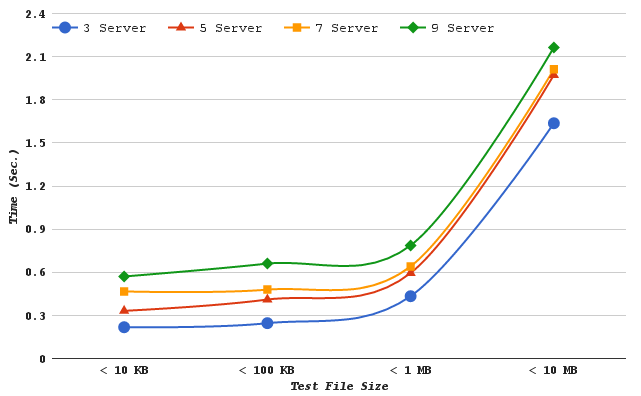
\includegraphics[width=.6\textwidth]{my_upload_not_same}
    \end{center}
\end{frame}

\begin{frame}{Experimental Results}
{The client device and SP are \alert{not} in the same network segment - My Method}
	\scriptsize
    \begin{table}[]
    \centering
    \caption{THE EXECUTION TIME OF \alert{DOWNLOAD} OPERATIONS (IN SEC.) (Account C)}
    \begin{tabular}{lcccc}
                         & 3 Server & 5 Server & 7 Server & 9 Server \\ \hline
        \textless 10 KB  & 0.263332 & 0.358435 & 0.590343 & 0.606110 \\ \hline
        \textless 100 KB & 0.270404 & 0.396497 & 0.567059 & 0.597088 \\ \hline
        \textless 1 MB   & 0.382264 & 0.590987 & 0.694622 & 0.846141 \\ \hline
        \textless 10 MB  & 0.823476 & 1.086515 & 1.208293 & 1.278169 \\ \hline
    \end{tabular}
    \end{table}
    \begin{center}
		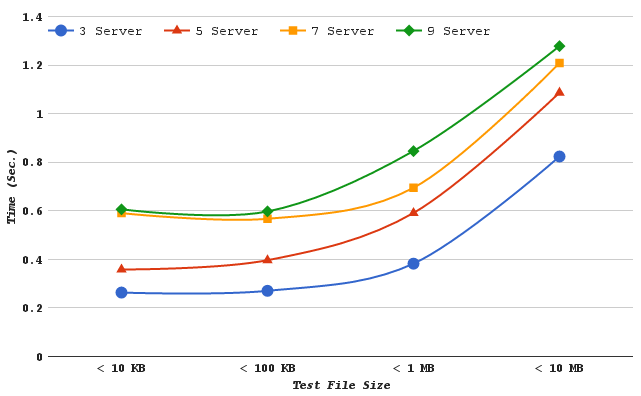
\includegraphics[width=.6\textwidth]{my_download_not_same}
    \end{center}
\end{frame}

\begin{frame}{Experimental Results}
{The client device and SP are \alert{not} in the same network segment - 2014 Cloud Com}
	\scriptsize
    \begin{table}[]
    \centering
    \caption{THE EXECUTION TIME OF \alert{UPLOAD} OPERATIONS (IN SEC.) (Account C)}
    \begin{tabular}{lccccl}
                         & sync 2   & sync 10  & sync 50  & sync 250 & sync 1250 \\ \hline
        \textless 10 KB  & 0.362766 & 0.411929 & 0.486570 & 0.862048 & 2.363091  \\ \hline
        \textless 100 KB & 0.377788 & 0.416367 & 0.508769 & 0.870478 & 2.453335  \\ \hline
        \textless 1 MB   & 0.556890 & 0.619318 & 0.698361 & 1.024154 & 2.665164  \\ \hline
        \textless 10 MB  & 1.525459 & 1.882746 & 1.929606 & 2.064955 & 3.566919  \\ \hline
    \end{tabular}
    \end{table}
    \begin{center}
		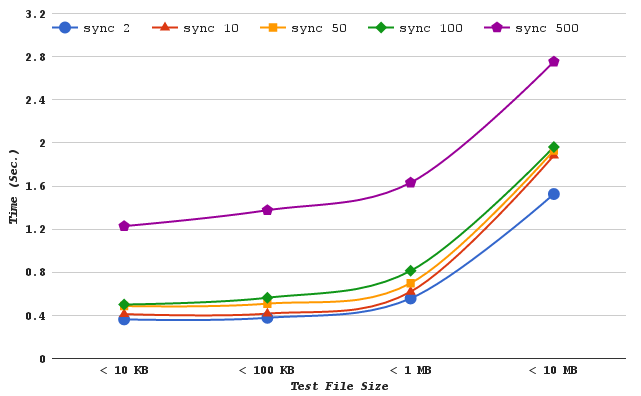
\includegraphics[width=.6\textwidth]{2014_upload_not_same}
    \end{center}
\end{frame}

\begin{frame}{Experimental Results}
{The client device and SP are \alert{not} in the same network segment - 2014 Cloud Com}
	\scriptsize
    \begin{table}[]
    \centering
    \caption{THE EXECUTION TIME OF \alert{DOWNLOAD} OPERATIONS (IN SEC.) (Account C)}
    \begin{tabular}{lccccl}
                         & sync 2   & sync 10  & sync 50  & sync 250 & sync 1250 \\ \hline
        \textless 10 KB  & 0.388520 & 0.374224 & 0.524074 & 1.202312 & 4.569076  \\ \hline
        \textless 100 KB & 0.427226 & 0.440348 & 0.584122 & 1.300710 & 4.590791  \\ \hline
        \textless 1 MB   & 0.574539 & 0.687956 & 0.772134 & 1.399860 & 4.684576  \\ \hline
        \textless 10 MB  & 0.933868 & 1.024385 & 1.145598 & 1.759997 & 4.945930  \\ \hline
    \end{tabular}
    \end{table}
    \begin{center}
		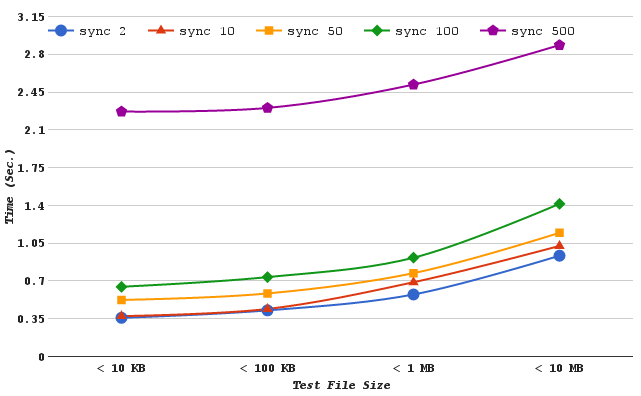
\includegraphics[width=.6\textwidth]{2014_download_not_same}
    \end{center}
\end{frame}

\begin{frame}{Experimental Results}
{The client device and SP are \alert{not} in the same network segment - UPLOAD operation}
	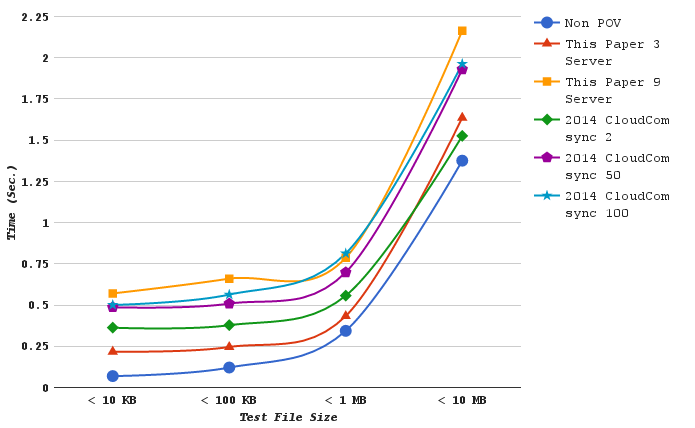
\includegraphics[width=\textwidth]{all_upload_not_same}
\end{frame}

\begin{frame}{Experimental Results}
{The client device and SP are \alert{not} in the same network segment - DOWNLOAD operation}
	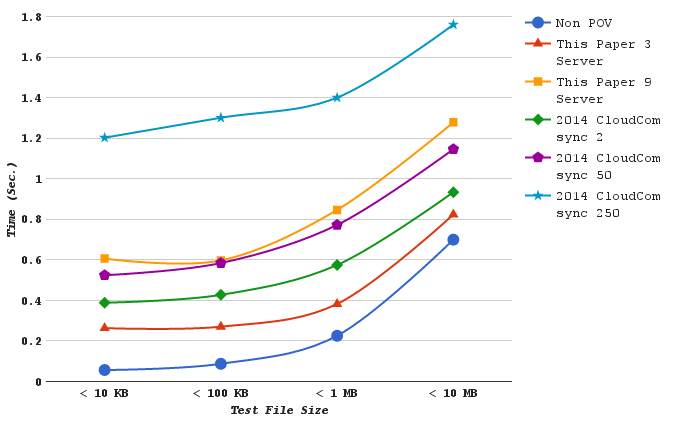
\includegraphics[width=\textwidth]{all_download_not_same}
\end{frame}

%OVERHEAD
\begin{frame}{Experimental Results}
{The client device and SP are \alert{not} in the same network segment - UPLOAD Overhead}
	\scriptsize
    \begin{table}[]
    \centering
    \caption{My Method - Non POV (IN SEC.) (Account C)}
    \begin{tabular}{lcccc}
                         & 3 Server & 5 Server & 7 Server & 9 Server \\ \hline
        \textless 10 KB  & 0.148290 & 0.262068 & 0.397382 & 0.501187 \\ \hline
        \textless 100 KB & 0.124676 & 0.289081 & 0.358134 & 0.539085 \\ \hline
        \textless 1 MB   & 0.089754 & 0.250948 & 0.297013 & 0.443104 \\ \hline
        \textless 10 MB  & 0.260857 & 0.596518 & 0.635884 & 0.788242 \\ \hline
    \end{tabular}
    \caption{2014 Cloud Com - Non POV (IN SEC.) (Account C)}
    \begin{tabular}{lccccl}
                         & sync 2   & sync 10  & sync 50  & sync 250 & sync 1250 \\ \hline
        \textless 10 KB  & 0.293493 & 0.342657 & 0.417297 & 0.792775 & 2.293818  \\ \hline
        \textless 100 KB & 0.256695 & 0.295274 & 0.387676 & 0.749385 & 2.332242  \\ \hline
        \textless 1 MB   & 0.213306 & 0.275733 & 0.354776 & 0.680570 & 2.321579  \\ \hline
        \textless 10 MB  & 0.149843 & 0.507130 & 0.553990 & 0.689340 & 2.191303  \\ \hline
    \end{tabular}
    \end{table}
\end{frame}

\begin{frame}{Experimental Results}
{The client device and SP are \alert{not} in the same network segment - DOWNLOAD Overhead}
	\scriptsize
    \begin{table}[]
    \centering
    \caption{My Method - Non POV (IN SEC.) (Account C)}
    \begin{tabular}{lcccc}
                         & 3 Server & 5 Server & 7 Server & 9 Server \\ \hline
        \textless 10 KB  & 0.206703 & 0.301806 & 0.533714 & 0.549481 \\ \hline
        \textless 100 KB & 0.183053 & 0.309147 & 0.479708 & 0.509738 \\ \hline
        \textless 1 MB   & 0.156698 & 0.365421 & 0.469057 & 0.620576 \\ \hline
        \textless 10 MB  & 0.123952 & 0.386991 & 0.508769 & 0.578646 \\ \hline
    \end{tabular}
    \caption{2014 Cloud Com - Non POV (IN SEC.) (Account C)}
    \begin{tabular}{lccccl}
                         & sync 2   & sync 10  & sync 50  & sync 250 & sync 1250 \\ \hline
        \textless 10 KB  & 0.331891 & 0.317594 & 0.467445 & 1.145683 & 4.512446  \\ \hline
        \textless 100 KB & 0.339875 & 0.352998 & 0.496772 & 1.213359 & 4.503441  \\ \hline
        \textless 1 MB   & 0.348973 & 0.462390 & 0.546568 & 1.174294 & 4.459011  \\ \hline
        \textless 10 MB  & 0.234344 & 0.324861 & 0.446074 & 1.060473 & 4.246406  \\ \hline
    \end{tabular}
    \end{table}
\end{frame}

%TIMES
\begin{frame}{Experimental Results}
{The client device and SP are \alert{not} in the same network segment - UPLOAD Overhead}
	\scriptsize
    \begin{table}[]
    \centering
    \caption{My Method / Non POV (IN SEC.) (Account C)}
    \begin{tabular}{lcccc}
                         & 3 Server & 5 Server & 7 Server & 9 Server \\ \hline
        \textless 10 KB  & 3.140669 & 4.783127 & 6.736478 & 8.234973 \\ \hline
        \textless 100 KB & 2.029588 & 3.387261 & 3.957507 & 5.451819 \\ \hline
        \textless 1 MB   & 1.261228 & 1.730382 & 1.864455 & 2.289650 \\ \hline
        \textless 10 MB  & 1.189629 & 1.433637 & 1.462254 & 1.573011 \\ \hline
    \end{tabular}
    \caption{2014 Cloud Com / Non POV (IN SEC.) (Account C)}
    \begin{tabular}{lccccl}
                         & sync 2   & sync 10  & sync 50  & sync 250  & sync 1250 \\ \hline
        \textless 10 KB  & 5.236767 & 5.946479 & 7.023971 & 12.444239 & 34.112817 \\ \hline
        \textless 100 KB & 3.119815 & 3.438406 & 4.201470 & 7.188500  & 20.259902 \\ \hline
        \textless 1 MB   & 1.620825 & 1.802520 & 2.032574 & 2.980794  & 7.756942  \\ \hline
        \textless 10 MB  & 1.108928 & 1.368657 & 1.402722 & 1.501113  & 2.592962  \\ \hline
    \end{tabular}
    ~\\
    ~\\
    ~\\
    \alert{Avg: 2.01 times, Max: 4.14 times}
    \end{table}
\end{frame}

\begin{frame}{Experimental Results}
{The client device and SP are \alert{not} in the same network segment - DOWNLOAD Overhead}
	\scriptsize
    \begin{table}[]
    \centering
    \caption{My Method / Non POV (IN SEC.) (Account C)}
    \begin{tabular}{lcccc}
                         & 3 Server & 5 Server & 7 Server  & 9 Server  \\ \hline
        \textless 10 KB  & 4.650108 & 6.329503 & 10.424700 & 10.703127 \\ \hline
        \textless 100 KB & 3.095611 & 4.539142 & 6.491742  & 6.835527  \\ \hline
        \textless 1 MB   & 1.694689 & 2.620022 & 3.079470  & 3.751199  \\ \hline
        \textless 10 MB  & 1.177195 & 1.553220 & 1.727308  & 1.827199  \\ \hline
    \end{tabular}
    \caption{2014 Cloud Com / Non POV (IN SEC.) (Account C)}
    \begin{tabular}{lccccl}
                         & sync 2   & sync 10  & sync 50  & sync 250  & sync 1250 \\ \hline
        \textless 10 KB  & 6.860769 & 6.608313 & 9.254478 & 21.231303 & 80.684047 \\ \hline
        \textless 100 KB & 4.890921 & 5.041151 & 6.687090 & 14.890653 & 52.555829 \\ \hline
        \textless 1 MB   & 2.547104 & 3.049914 & 3.423100 & 6.205999  & 20.768135 \\ \hline
        \textless 10 MB  & 1.335005 & 1.464403 & 1.637682 & 2.515992  & 7.070423  \\ \hline
    \end{tabular}
    ~\\
    ~\\
    ~\\
    \alert{Avg: 2.93 times, Max: 7.53 times}
    \end{table}
\end{frame}